\documentclass[12pt,xcolor=dvipsnames]{beamer}
\usetheme{CambridgeUS}
\usecolortheme{whale}
\setbeamercolor{block title}{use=structure,fg=white,bg=blue!75!black}  
\setbeamercolor{block body}{use=structure,fg=black,bg=blue!5!white}
\setbeamercolor{frametitle}{bg=Blue}

\usepackage{hyperref}   
\usepackage{url}
\hypersetup{urlcolor=red}

\renewcommand{\bibname}{References}
\setbeamertemplate{bibliography item}{[\theenumiv]}

\usepackage{multicol}
\usepackage{multirow}
\usepackage{verbatim} 
\usepackage{graphics}
\usepackage{graphicx}


\usepackage{chapterbib}
%\usepackage{tikz}
%\usepackage{pgfplots}
%\usepgfplotslibrary{groupplots} 
%\usepackage{pgf, pgfarrows, pgfnodes}
\usepackage{lscape}
\usepackage{longtable}
\usepackage{float}
\usepackage{url}
\usepackage{multicol}
\usepackage{color}
\usepackage{multirow}
\usepackage{listings}
\usepackage{subfigure}
\usepackage{tabularx,ragged2e,booktabs,caption}
\usepackage{placeins}
\usepackage[toc,page]{appendix}


%Basic Information
\title{Load Testing and Benchmarking for BigData}
\author{Aayush Agrawal, Sunil Raiyani, Jayam Modi}

%--------------------------------------------------------------------------------------
%               TITLE PAGE (Slide 1)
%--------------------------------------------------------------------------------------
\begin{document}
 


\begin{frame}
\titlepage
\end{frame}
%--------------------------------------------------------------------------------------


%--------------------------------------------------------------------------------------
%               Outline
%--------------------------------------------------------------------------------------
\begin{frame}
\frametitle{Outline}
\begin{multicols}{2}
\tableofcontents[hideallsubsections]
\end{multicols}
\end{frame}

%--------------------------------------------------------------------------------------
%               Slide 1: Topic 1
%--------------------------------------------------------------------------------------

\begin{frame}[t]
\frametitle{Aim of the Project}
The aim of the project is Load Testing and Benchmarking for BigData. 
\newline
\newline
The major task is to setup a distributed file system on a cluster, test the data and query processing capacity 
of the system using BigBench and predict the performance of the system for larger data sets.
\end{frame}


\section{Important Terms}
\begin{frame}[t]
\frametitle{Important Terms}

\begin{enumerate}
 \item \textbf{Load Testing} -  It involves testing the system by steadily increasing the load on the system till it reaches
its threshold limit
 \item \textbf{BenchMarking} - It is the process of comparing the performance metrics of own systems with the industry 
 standards.
 \item \textbf{BigData} - It is a term that covers data sets so large and complex that it becomes impossible to process them using
 on-hand database management tools and traditional data processing applications.
\end{enumerate}


\end{frame}
\section{Distributed Processing Tools Used}
\begin{frame}[t]
\frametitle{Distributed Processing Tools Used}
\begin{itemize}
 \item \textbf{Hadoop}
 \newline\noindent
Apache Hadoop \cite{hadoop} provides a Distributed file system named HDFS which is a platform to store huge
amounts of data divided into blocks across multiple hosts and a MapReduce engine which performs
the processing of BigData
\newline
\newline
 \item \textbf{Hive}
 \newline\noindent
Apache Hive, as reported in \cite{hive} , is a data warehouse infrastructure built on top of
hadoop for providing data analysis and querying features

\end{itemize}

\end{frame}

\begin{frame}[t]
\begin{itemize}
\item \textbf{Ganglia}
 \newline\noindent
Ganglia, as reported in \cite{ganglia} ,is a scalable distributed monitoring system for high-performance computing
systems such as clusters and Grids
\newline
\newline
 \item \textbf{BigBench}
 \newline\noindent
\cite{ghazal} introduces BigBench as an industry standard benchmark for big data analytics. All the major characteristics in the
lifecycle of a big data system are covered in BigBench which is an end-to-end benchmark.
\end{itemize}
 
\end{frame}

\section{Procedure of the Experiment}
\begin{frame}[t]
\frametitle{Block Diagram}
\begin{figure}[h]
 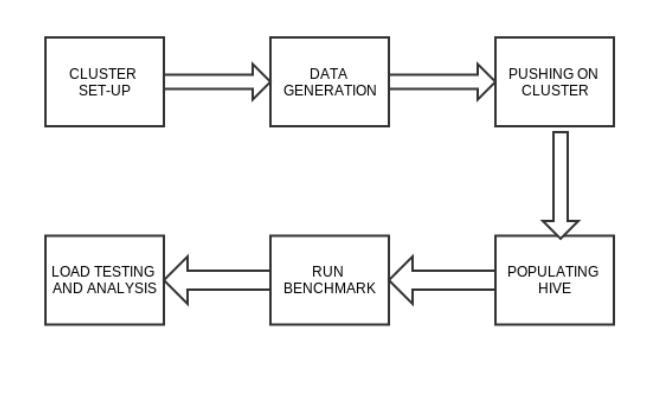
\includegraphics[width=10cm]{block_diagram.jpeg}
\caption{Average Query Response Times for different data sizes \label{block}}
\end{figure}
\end{frame}


\begin{frame}[t]
\frametitle{Experimental Set-up}
\begin{itemize}
  \item \textbf{Namenode} : [Dual CPU] Intel Xeon E5-2620 v2 @ 2.10GHz server with 8 * 16384 MB @1600 MHz Samsung Synchronous DDR3 RAM and 
 LSI MegaRAID SAS 9240-4i disk with 6 Gb/s SATA on each of 4 internal ports. The operating system is Ubuntu-Linux 12.04 Server.
 \item \textbf{Datanode} : Intel(R) Core(TM)2 CPU E7500  @ 2.93GHz commodity machine with 2048 MB @800MHz Synchronous DDR RAM and Seagate's
 500GB 7200 RPM 3.5" Internal Hard Drive with 16MB Cache and 3 Gb/s SATA. The operating system is Ubuntu-Linux 14.04 Desktop.
\end{itemize}

The \textbf{network} connecting namenode and datanodes is a 100Mb/s Wired Ethernet.
\end{frame}

\begin{frame}[t]
\frametitle{Data Generation and Workload Customization}
\begin{itemize}
 \item PDGF generator at \cite{bigbenchgit}, is used to generate data.
 \item Modification of the workload to suit our experiment.
 \item Data is first generated on the local machine.
 \item Pushed data onto the cluster.
 \item Populated hive tables using this data.
 \item Chose only 9 queries out of 30 from \cite{bigb} as most of them generated empty set results on the synthetically generated data.
\end{itemize}
\end{frame}

\begin{frame}[t]
\frametitle{Query Distribution in Customized Workload}
The distribution of queries among different types of data is as follows:
\begin{center}
\begin{tabular}{|l|c|c|}\hline
Query-Type & Queries & Percentage\\\hline
Declarative & 3,6,7,8 & 44.4\% \\
Mixed & 2,5,9 & 33.4\% \\
Procedural & 1,4 & 22.2\%\\\hline
\end{tabular}
\end{center}

\begin{center}
\begin{tabular}{|l|c|c|}\hline
 Data-Type & Queries & Percentage\\\hline
 Structured & 3,6,7,8,9 & 55.5\%\\
 Semi-Structured & 1,2 & 22.2\%\\
 Unstructured & 4,5 & 22.3\%\\\hline
\end{tabular}

\end{center}

\end{frame}

\section{Load Testing}
\begin{frame}[t]
\frametitle{Load Testing}
The following table lists the average query response time(in sec) for different data sizes(in GB) obtained experimentally:
\begin{center}
\begin{tabular}{|c|c|c|c|}\hline
\multirow{2}{*}{Data Size} & \multicolumn{3}{c|}{Query Response Time (sec)}\\
\cline{2-4}
& 2 DataNodes & 3 DataNodes & 4 DataNodes\\\hline
1 & 293 & 188 & 172\\
5 & 358 & 317 & 275\\
10 & 1125 & 617 & 530\\
25 & - & 1154 & 1040\\
40 & - & 1451 & 1682\\
45 & - & 1793 & 1924\\
50 & - & 1956 & 2205\\
75 & - & 3054 & 3029\\
100 & - & 4491 & 4312\\\hline
\end{tabular}
\end{center}
\end{frame}

\begin{frame}
\frametitle{Load Testing}
 The figures \ref{barcomp} and \ref{linecomp} indicate the comparison between the average query response times for 3 datanodes and 4 datanodes.
\begin{figure}[h]
 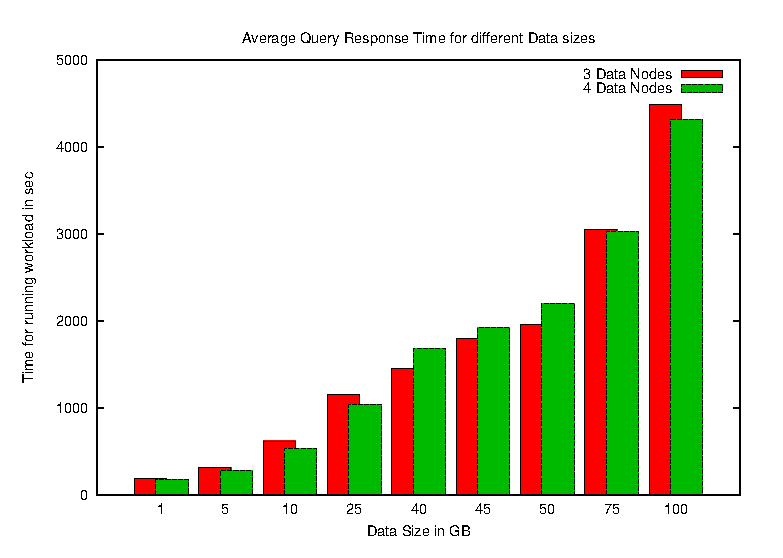
\includegraphics[width=7cm]{bar_comparison.eps}
\caption{Average Query Response Times for different data sizes \label{barcomp}}
\end{figure}
\end{frame}

\begin{frame}
\frametitle{Load Testing}
\begin{figure}[h]
 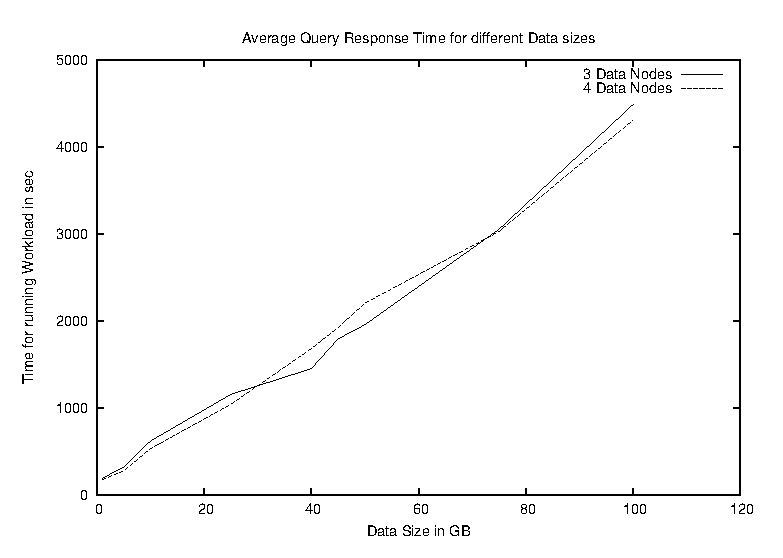
\includegraphics[width=8cm]{line_comparison.eps}
\caption{Average Query Response Times for different data sizes \label{linecomp}}
\end{figure}
\end{frame}

\begin{frame}[t]
\frametitle{Observations}
\begin{itemize}
 \item Initially, the average query response time using 4 datanodes was less than that using 3 datanodes.
 \item Gradually, as the data size increased, the time for 4 datanodes was more in comparison to that for 3 datanodes
 \item Furthermore, when the data size was increased further, the average response time behavior becomes same as it was initially.
\end{itemize}
\end{frame}

\begin{frame}[t]
\frametitle{Interpretation of Results}
\begin{itemize}
 \item The average query response time is affected by a combination of multiple factors such as:
\begin{enumerate}
 \item Division and distribution of work of queries across multiple nodes on the HDFS system.
 \item Time to transfer intermediate results over the network.
 \item Degree of swapping that takes place.
\end{enumerate}
\item Network transfer time is not significant for smaller intermediate results of small data size.
\item For larger data size, swapping at each node and network transfer time dominates faster computation 
    since intermediate results are also large. This brings the change of behaviour observed in the graph.
\end{itemize}

\end{frame}

\begin{frame}[t]
\frametitle{Interpretation of Results}
\begin{itemize}
\item Data is distributed over more number of nodes and hence network transfer is also more.
\item With further increase in data size, swapping becomes constant. So more distribution of workload dominates other factors.
\item Computations become faster and behaviour of average response time becomes same as before.
\newline
\end{itemize}
Apart from these, there may be several other factors involved which affect the average response time of the system. 
Further investigation is required for analyzing this behavior.
\end{frame}


\section{Predictive Analysis}
\begin{frame}[t]
\frametitle{Predictive Analysis}
We have drawn a mean line which can be extrapolated to predict the scale factors for larger data sizes.
The figures \ref{sf3} and \ref{sf4} indicate the scale factor for change in  query response time w.r.t 1 GB of data.
\begin{figure}[h]
 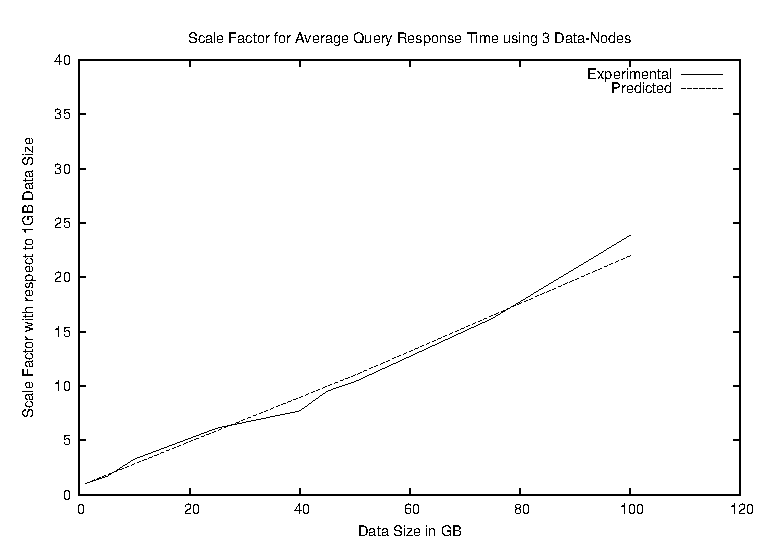
\includegraphics[width=7cm]{sf3.eps}
\caption{Scale factor for 3 datanodes \label{sf3}}
\end{figure}
\end{frame}

\begin{frame}[t]
\frametitle{Predictive Analysis}
\begin{figure}[h]
 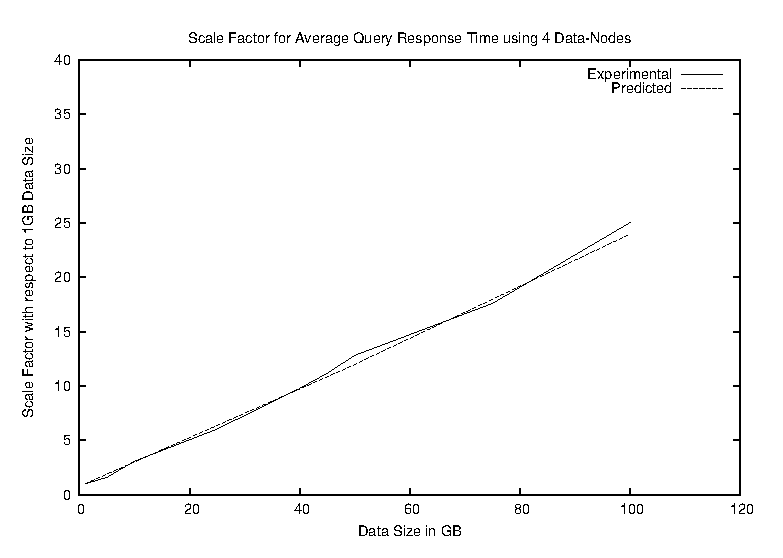
\includegraphics[width=8cm]{sf4.eps}
\caption{Scale factor for 4 datanodes \label{sf4}}
\end{figure}
\end{frame}

\begin{frame}[t]
\frametitle{Predictive Analysis}
%The following table shows the deviation of predicted results from the experimental results:
\begin{center}
\captionof{table}{Error in Predicted time w.r.t Experimental time for 3 Datanodes}
\begin{tabular}{|c|c|c|c|}\hline
\multirow{2}{*}{Data Size} & \multicolumn{3}{c|}{Time (sec)}\\
\cline{2-4}
& Experimental & Predicted & Deviation\\\hline
1 & 188 & 188 & 0\\
5 & 317 & 338 & 21\\
10 & 617 & 526 & 91\\
25 & 1154 & 1090 & 64\\
40 & 1451 & 1654 & 103\\
45 & 1793 & 1842 & 49\\
50 & 1956 & 2030 & 74\\
75 & 3054 & 2970 & 84\\
100 & 4491 & 3910 & 481\\\hline
\end{tabular}
\end{center}
\end{frame}

\begin{frame}[t]
 \frametitle{Predictive Analysis}
\begin{center}
\captionof{table}{Error in Predicted time w.r.t Experimental time for 4 Datanodes}
\begin{tabular}{|c|c|c|c|}\hline
\multirow{2}{*}{Data Size} & \multicolumn{3}{c|}{Time (sec)}\\
\cline{2-4}
& Experimental & Predicted & Deviation\\\hline
1 & 172 & 170 & 2\\
5 & 275 & 321 & 46\\
10 & 530 & 510 & 20\\
25 & 1040 & 1078 & 38\\
40 & 1682 & 1646 & 32\\
45 & 1924 & 1835 & 79\\
50 & 2205 & 2024 & 181\\
75 & 3029 & 2970 & 59\\
100 & 4312 & 3916 & 396\\\hline
\end{tabular}
\end{center}
\end{frame}

\section{Progress of the project}
\begin{frame}[t]
\frametitle{Initial Tasks}
 The following tasks have been completed:
\begin{itemize}
 \item  Study of the TPC-H and TPC-C benchmarks.
 \item  Study of the research papers. \cite{paper} \cite{paper1}
 \item  Hadoop and Hive installation.
 \item  Working with BigBench.
 \item  Load testing experiments.
\end{itemize}
\end{frame}

\section{Future Scope}
\begin{frame}[t]
\frametitle{Future Scope}
 The following work is considered for future:
\begin{itemize}
 \item  Run the experiment for clusters of larger size and try to determine the optimum size of cluster of the given
	configuration of nodes to manage a particular data-set size.
 \item Analyze other parameters affecting the average query response time of the system.
 \item  Open Source Release of our customized version of BigBench.
\end{itemize}
\end{frame}

%---------------------------------------------------------------------------------------
%     Final Slide - References
%--------------------------------------------------------------------------------------
\section{References }
\frametitle{References }
\begin{frame}[allowframebreaks]{References}
\bibliographystyle{ieeetr}
\bibliography{biblio}
%\bibliography{biblio}




\end{frame}
\end{document}
